\documentclass{beamer}
\usepackage{amsmath}
\usepackage{graphicx}
\graphicspath{{./figures/}}

\usepackage{tikz}
\usepackage{pgfplots}
\pgfplotsset{compat=1.18}

\usetheme{Boadilla}
\usecolortheme{seahorse}

\title{Probabilities and Random Variables}
\author{Vasilis Gkolemis}
\institute{ATHENA RC | HUA}
\date{June 2025}

\begin{document}



\begin{frame}
  \titlepage
  \vfill
  \footnotesize
  \textcopyright\
  Vasilis Gkolemis, 2025. Licensed under CC BY 4.0.
\end{frame}

\begin{frame}{Contents}
  \tableofcontents
\end{frame}


\begin{frame}{Helping Material}
  \begin{itemize}
    \item \textbf{Primer on Probabilistic Modeling} \url{https://www.inf.ed.ac.uk/teaching/courses/pmr/22-23/assets/notes/probabilistic-modelling-primer.pdf}
  \end{itemize}
\end{frame}


\section{Informal Introduction to Probability Theory}

\begin{frame}{}
    \begin{center}
        \textcolor{blue}{\bfseries \emph{We will start at the very beginning: \\
The realm of probability theory!}}
    \end{center}
\end{frame}


\begin{frame}{}\begin{minipage}{.35\linewidth}
     Quick set theory reminder:
\end{minipage}%
\begin{minipage}{.65\linewidth}
    \vspace{-1.2cm}
  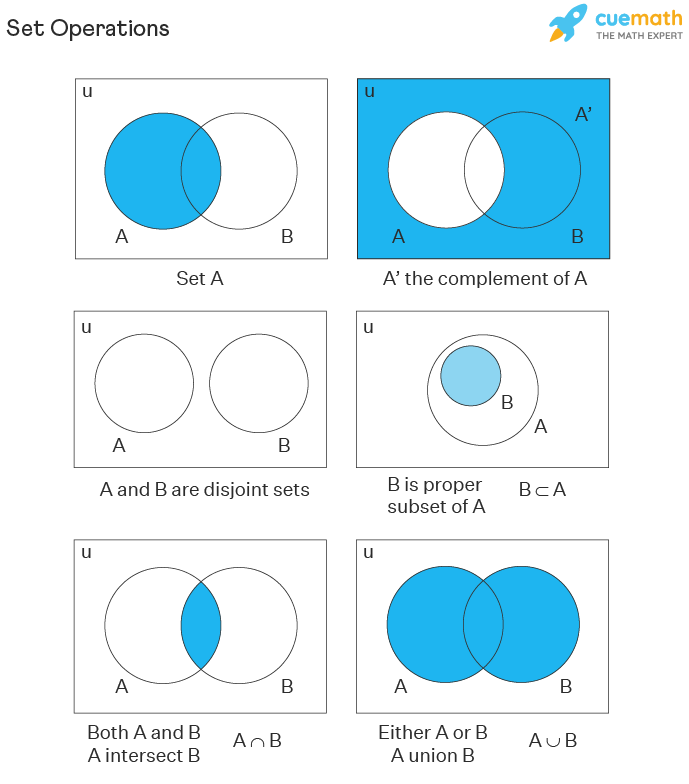
\includegraphics[height=\paperheight]{graphics/SetOperationsold.png}
\end{minipage}
\end{frame}

\begin{frame}{}
    \begin{center}
        \textcolor{blue}{\textbf{\Large{QUESTION:}}}\bigskip\\

        \emph{\Large What is your understanding of the term "probability"?}
    \end{center}
  \end{frame}

\begin{frame}{}
\begin{center}
        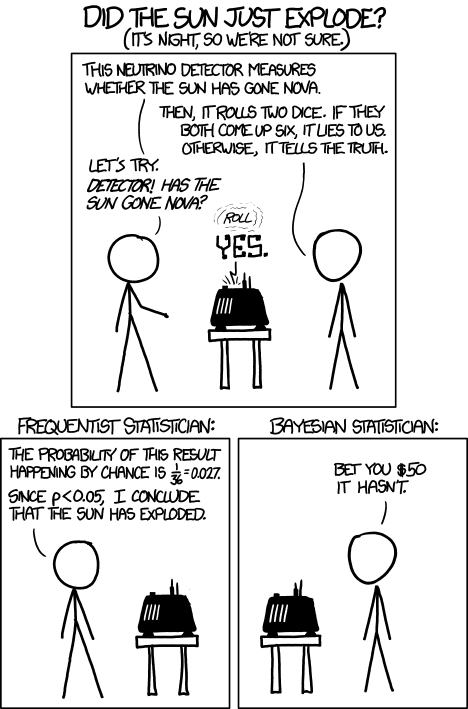
\includegraphics[height=.9\paperheight]{graphics/frequentists_vs_bayesians.png}
\end{center}
\end{frame}

% Slide 1 - Probability
\begin{frame}{What is Probability?}
\begin{itemize}
  \item Probability is a number between 0 and 1.
  \item It tells us how likely an event is to happen.
\end{itemize}

\vspace{1cm}

\begin{center}
\begin{tabular}{|c|c|}
\hline
Event & Probability \\
\hline
Heads in a coin flip & 0.5 \\
Rolling a 3 on a die & $1/6$ \\
Sun rises tomorrow & 1 \\
Finding a unicorn & 0 \\
\hline
\end{tabular}
\end{center}

\vspace{0.5cm}
\begin{block}{Interpretation}
\centering
Probability helps us reason about uncertainty.
\end{block}
\end{frame}


\begin{frame}{What is a Probability Space?}
  A probability space is a triple $(\Omega, \mathcal{F}, P)$:
  \vspace{0.5cm}
\begin{enumerate}
  \item \textbf{Sample space} $\Omega$: the set of all possible outcomes.
  \item \textbf{Events} $\mathcal{F}$: a collection of subsets of $\Omega$ (events).
  \item \textbf{Probability function} $P$: a function $P: \mathcal{F} \rightarrow [0,1]$ assigning probabilities to events.
\end{enumerate}

\vspace{0.5cm}
\begin{block}{Example: Rolling a Die}
\begin{itemize}
  \item $\Omega = \{1, 2, 3, 4, 5, 6\}$
    \begin{itemize}
      \item they are outcomes $\Rightarrow$ we could write $\Omega = \{a, b, c, d, e, f\}$
    \end{itemize}
  \item Event $A$: any even number $\Rightarrow A = \{2, 4, 6\}$
    \begin{itemize}
      \item $A \subseteq \Omega$, e.g. if $\Omega = \{a, b, c, d, e, f\}$ then $A = \{b, d, f\}$
    \end{itemize}
  \item $P(\{2\}) = P(\{4\}) = P(\{6\}) = \frac{1}{6} \Rightarrow P(A) = \frac{3}{6}$
\end{itemize}
\end{block}
\end{frame}

% Slide 3 - Random Variable
\begin{frame}{What is a Random Variable?}
  \begin{itemize}
  \item A \textbf{random variable} $X$:
    \begin{itemize}
      \item maps outcomes to numbers, i.e., is a \textbf{function} $X: \Omega \rightarrow \mathbb{R}$.
      \item gives \textit{a numerical view of the sample space}
      \item we can say "$P$ that $X$ is even" instead of directly referring to $\Omega$.
    \end{itemize}
\end{itemize}

\vspace{0.4cm}
\begin{block}{Example: Rolling a Die}
$\Omega = \{a, b, c, d, e, f\}$ are outcomes; $X$ maps them to numbers:
\[
X(a)=1,\ X(b)=2,\ X(c)=3,\ X(d)=4,\ X(e)=5,\ X(f)=6
\]
So the event $\{b, d, f\} \subseteq \Omega$ becomes $X$ is an even number.
\end{block}
\vspace{0.2cm}
\begin{center}
\textit{A random variable is like a lens: it translates raw outcomes into numbers.}
\end{center}
\end{frame}


% Slide 4 - Distribution
\begin{frame}{What is a Distribution?}
\begin{itemize}
  \item A \textbf{distribution} tells us how likely each value of a random variable is.
  \item It is a function: maps values of the random variable to probabilities.
\end{itemize}

\vspace{0.3cm}
\begin{block}{Example: Die Roll}
Let $X$ be the result of rolling a fair 6-sided die:
\[
P(X = k) = \frac{1}{6}, \quad \text{for } k = 1,2,3,4,5,6
\]
Uniform distribution over $\{1, 2, 3, 4, 5, 6\}$
\end{block}

\vspace{0.2cm}
\begin{center}
\textit{The distribution describes the behavior of the random variable.}
\end{center}

\end{frame}

\begin{frame}{What is a Distribution?}
\begin{itemize}
  \item A \textbf{distribution} tells us how likely each value of a random variable is.
  \item It is a function: maps values of the random variable to probabilities.
\end{itemize}

\vspace{0.3cm}
\begin{center}
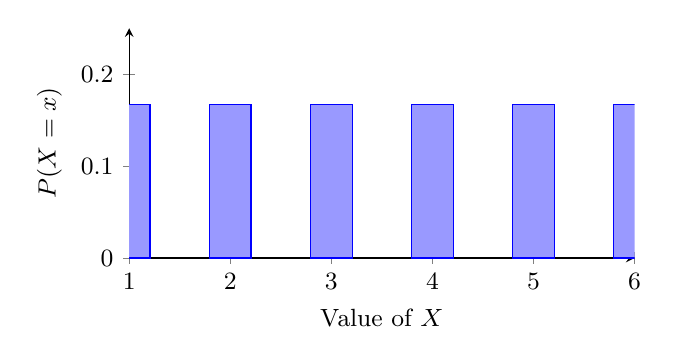
\begin{tikzpicture}
  \begin{axis}[
    width=8cm,
    height=4.5cm,
    ybar,
    bar width=15pt,
    ymin=0,
    ymax=0.25,
    ylabel={$P(X = x)$},
    xlabel={Value of $X$},
    xtick={1,2,3,4,5,6},
    ytick={0,0.1,0.2},
    yticklabels={0, 0.1, 0.2},
    enlarge x limits=0.15,
    axis lines=left,
    every axis/.append style={font=\small}
  ]
  \addplot+[fill=blue!40] coordinates {
    (1,0.1667) (2,0.1667) (3,0.1667) (4,0.1667) (5,0.1667) (6,0.1667)
  };
  \end{axis}
\end{tikzpicture}
\end{center}
\end{frame}

% Slide 5 - Summary: From Outcomes to Distributions
\begin{frame}{From Outcomes to Distributions}

\begin{block}{The Full Chain}
\(
(\Omega, \mathcal{F}, P)
\quad \xrightarrow{\text{Random Variable }} \quad
X: \Omega \rightarrow \mathbb{R}
\quad \xrightarrow{\text{Distribution}} \quad
P(X = x)
\)
\end{block}

\vspace{0.5cm}

\begin{block}{Do we need the full chain?}
\begin{itemize}
  \item Only in formal probability theory.
  \item In applications and modeling, we start directly from a \textbf{distribution}.
    \begin{itemize}
    \item Uniform: $P(X = k) = \frac{1}{n}$ for $k \in \{1, \dots, n\}$
    \item Bernoulli: $P(X = 1) = p,\quad P(X = 0) = 1-p$
    \item The underlying $(\Omega, \mathcal{F}, P)$ is abstract or implicit.
    \end{itemize}
\end{itemize}
\end{block}


\vspace{0.3cm}
\begin{center}
  \textit{In probabilistic modeling we often start directly from a distribution, without explicitly defining the sample space or events.}
\end{center}

\end{frame}


% \section{Formal Introduction to Probability Theory}


% \begin{frame}{Mathematics is here to help!}
%     \begin{itemize}
%         \item So is there no ''true'' definition of probability?!
%         \item Actually, there are two equivalent ways of formalizing the concept of probability:\bigskip\\\begin{itemize}
%             \item \textcolor{blue}{Cox's theorem}\vspace{-.1cm}\\
%             \item \textcolor{blue}{The axioms of Kolmogorov (probability axioms)} \\
%             $\rightarrow$ \emph{what we will focus on, since much more popular.}
%         \end{itemize}
%         \end{itemize}
%         \end{frame}

% \begin{frame}[allowframebreaks]{Kolmogorov axioms - heuristic version}
%     \begin{minipage}{.6\linewidth}
%         \begin{itemize}
%             \item The axiomatic foundations of modern probability theory were laid \textcolor{blue}{only as recently as 1933}!
%             \item Specifically, they were published in the book \emph{Foundations of the Theory of Probability} by Andrey Kolmogorov.
%         \end{itemize}
%     \end{minipage}%
%     \begin{minipage}{.4\linewidth}
%         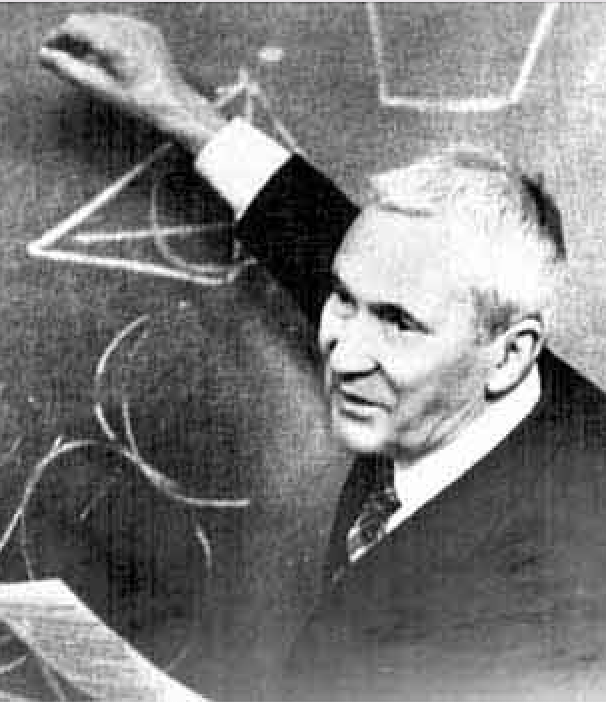
\includegraphics[width=\linewidth]{graphics/Kolmogorov.png}
%     \end{minipage}\,\\\pagebreak
%     \textbf{Heuristically}, for an event space $\mathcal{S}$, i.e. the set of all possible events, the axioms state the following:\bigskip\\

%     \hspace*{1cm}\begin{minipage}{.9\linewidth}
%      \begin{itemize}
%         \item[Axiom 1:] For any event $E$, the probability of $E$ is greater or equal to zero.
%         \item[Axiom 2:] The probability of the union of all events equals $1$.
%         \item[Axiom 3:] For a countable sequence of mutually exclusive events $E_1,E_2,E_3,...$ the probability of any of these events occurring is equal to the sum of each of the events occurring.
%     \end{itemize}
%     \end{minipage}

% \end{frame}

\section{Properties of a Probability Distribution}

\begin{frame}{What Can We Do With a Distribution?}

A probability distribution allows us to:

\vspace{1em}
\begin{enumerate}
  \item \textbf{Define a probability density function (PDF)} or a \textbf{probability mass function (PMF)}.
  \begin{itemize}
    \item Gives the relative likelihood of each outcome.
  \end{itemize}

  \item \textbf{Define a cumulative distribution function (CDF).}
  \begin{itemize}
    \item $F(x) = P(X \leq x)$, accumulates probability up to $x$.
  \end{itemize}

  \item \textbf{Summarize properties of the distribution.}
  \begin{itemize}
    \item Most important: \textbf{expected value (mean)} and \textbf{variance (spread)}.
    \item Also: skewness, kurtosis, entropy, etc.
  \end{itemize}

  \item \textbf{Sample from the distribution.}
  \begin{itemize}
    \item Generate artificial data consistent with the modeled uncertainty.
  \end{itemize}
\end{enumerate}

\end{frame}

\subsection{PDF and PMF}

\begin{frame}{PMF and PDF}

\textbf{Probability Mass Function (PMF) -- Discrete Random Variables:}
\[
P(X = x) = p(x)
\]
\begin{itemize}
  \item Gives the probability that the random variable equals a specific value.
  \item Probabilities add up over all possible values and sum to 1.
\end{itemize}

\vspace{1em}

\textbf{Probability Density Function (PDF) -- Cont. Random Variables:}
\[
P(a \leq X \leq b) = \int_a^b p(x) \, dx
\]
\begin{itemize}
  \item Gives the \textit{density} of the random variable around a point; probabilities come from areas under the curve.
  \item The value at a single point is not a probability (can be $>1$).
\end{itemize}

\end{frame}


\begin{frame}{Cumulative Distribution Function (CDF)}

\textbf{Cumulative Distribution Function (CDF):}
\[
F(x) = P(X \leq x)
\]
\begin{itemize}
  \item Gives the probability that the random variable takes a value less than or equal to $x$.
  \item For discrete variables: a step function; for continuous variables: a smooth, increasing curve.
\end{itemize}

\vspace{1em}

\textbf{Properties:}
\begin{itemize}
  \item $F(x)$ is non-decreasing and satisfies: $\lim_{x \to -\infty} F(x) = 0$, $\lim_{x \to +\infty} F(x) = 1$.
  \item For continuous variables: $p(x) = \frac{d}{dx} F(x)$.
\end{itemize}

\end{frame}

\subsection{Expected Value}
\begin{frame}{Expectation}
\textbf{Expectation} is a property of a probability distribution, representing a probability-weighted average.

\vspace{1em}
\textbf{Definition:} For a function $f$ of an outcome $x$,

\begin{center}
\begin{tabular}{cc}
\textbf{Discrete:} & \textbf{Continuous:} \\
$\displaystyle \mathbb{E}[f(x)] = \sum_{i=1}^{I} p_i f(a_i)$ &
$\displaystyle \mathbb{E}[f(x)] = \int_{-\infty}^{\infty} f(x) \, p(x) \, dx$
\end{tabular}
\end{center}

\vspace{1em}
\begin{itemize}
  \item Subscript $P(x)$ often dropped when context is clear.
  \item Notation variants: $\mathbb{E}[f]$, $\mathcal{E}[f]$, $\langle f \rangle$.
  \item If $f(x) = x$, then $\mathbb{E}[x]$ is the \textbf{mean}.
\end{itemize}
\end{frame}


\begin{frame}{Properties of Expectations}
\textbf{1. Linearity:}
\[
\mathbb{E}[f(x) + g(x)] = \mathbb{E}[f(x)] + \mathbb{E}[g(x)], \quad
\mathbb{E}[c f(x)] = c \, \mathbb{E}[f(x)]
\]

\textbf{2. Constant Rule:}
\[
\mathbb{E}[c] = c \sum_{i=1}^{I} p_i = c
\]
Because probabilities sum to one.

\textbf{3. Independence Rule:}
\[
\mathbb{E}[f(x) g(y)] = \mathbb{E}[f(x)] \, \mathbb{E}[g(y)]
\]
If $x$ and $y$ are independent.

\vspace{1em}
\textit{Exercise: Prove the independence rule.}
\end{frame}


\begin{frame}{The Mean (Expected Value)}
\textbf{The mean} of a distribution is the \textit{expected value} of numerical outcomes:
\[
\mu = \mathbb{E}[x] = \sum_{i=1}^{I} p_i a_i
\]

\vspace{1em}
\textbf{Examples:}
\begin{itemize}
  \item \textbf{Six-sided die:}
  \[
  \mathbb{E}[x] = \frac{1}{6}(1 + 2 + 3 + 4 + 5 + 6) = 3.5
  \]
  (Note: not an actual outcome, but a statistical average.)

  \item \textbf{Bernoulli trial (1 with probability $p$):}
  \[
  \mathbb{E}[x] = p \cdot 1 + (1 - p) \cdot 0 = p
  \]
\end{itemize}

\vspace{1em}
\textbf{Change of units:} If $x$ is in metres and we want cm:
\[
\mathbb{E}[100x] = 100 \, \mathbb{E}[x]
\]
\end{frame}


\subsection{Variance}
\begin{frame}{The Variance}
\textbf{Variance} measures the average squared distance from the mean:
\[
\text{var}[x] = \sigma^2 = \mathbb{E}\left[(x - \mu)^2\right] = \mathbb{E}[x^2] - \mathbb{E}[x]^2
\]
where $\mu = \mathbb{E}[x]$ is the mean.

\vspace{1em}
\textbf{Properties:}
\begin{itemize}
  \item $\text{var}[cx] = c^2 \, \text{var}[x]$
  \item If $x$ and $y$ are independent: \\
    $\text{var}[x + y] = \text{var}[x] + \text{var}[y]$
\end{itemize}

\vspace{0.5em}
\textbf{Standard deviation:} $\sigma = \sqrt{\text{var}[x]}$
Same units as $x$, often used as a measure of spread.
\end{frame}

\begin{frame}{Variance: Change of Units and Normalization}
\textbf{Change of Units:}
\begin{itemize}
  \item If $x$ is in metres, then $x^2$ is in $\text{m}^2$.
  \item Variance changes with units: \\
  $\text{var}[100x] = 100^2 \, \text{var}[x]$
\end{itemize}

\vspace{1em}
\textbf{Normalization:}
\begin{itemize}
  \item Given mean $\mu$ and variance $\sigma^2$, to normalize $x$: \\
    \[
    x_{\text{norm}} = \frac{x - \mu}{\sigma} \quad \Rightarrow \quad \mathbb{E}[x_{\text{norm}}] = 0, \quad \text{var}[x_{\text{norm}}] = 1
    \]
\end{itemize}

\textit{Note: Variance has different units from $x$, so it's not always directly interpretable.}
\end{frame}

\subsection{Sampling}

\begin{frame}{Sampling from a Distribution}
\textbf{Sampling} means generating random values that follow a given probability distribution.

\vspace{1em}
\textbf{Notation:} If $x$ is a random variable sampled from distribution $P$, we write:
\[
x \sim P
\]

\vspace{1em}
\textbf{Key Points:}
\begin{itemize}
  \item Some distributions are easy to sample from (e.g., Bernoulli, Gaussian), others require advanced methods.
  \item Sampling allows to \textit{easily} approximate important properties of the distribution:
    \begin{itemize}
      \item Mean: $\mathbb{E}[x] \approx \frac{1}{N} \sum_{i=1}^{N} x_i$ for $N$ samples.
      \item Variance: $\text{var}[x] \approx \frac{1}{N-1} \sum_{i=1}^{N} (x_i - \mathbb{E}[x])^2$.
      \end{itemize}
      \end{itemize}
\end{frame}


\section{Important Distributions}

\subsection{Bernoulli distribution}

\begin{frame}{Bernoulli Distribution}
  \textbf{Definition:} Models a procedure with two outcomes: success (1) an failure (0).
  \textbf{Example: Coin toss}: Toss a biased coin with probability \(p=0.7\) of landing heads (success).
  \vspace{0.5em}
  \[
    X \sim \text{Bernoulli}(p), \quad P(X=1) = p, \quad P(X=0) = 1-p
  \]

  \begin{columns}[T] % align columns at the top
    \begin{column}{0.48\textwidth}
      \textbf{Properties:}
      \begin{itemize}
        \item Mean: \( \mathbb{E}[X] = p = 0.7 \)
        \item Variance: \( \mathrm{Var}(X) = p(1-p) = 0.21 \)
      \end{itemize}
    \end{column}

    \begin{column}{0.48\textwidth}
      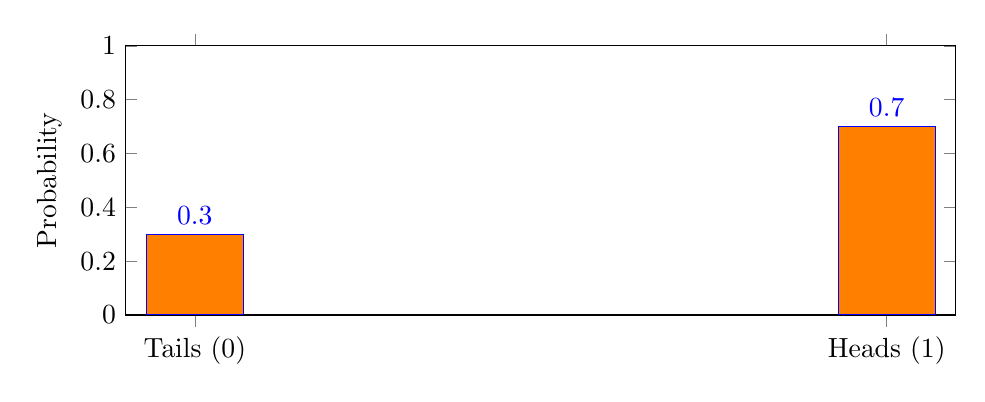
\begin{tikzpicture}
        \begin{axis}[
          ybar,
          bar width=35pt,
          width=\linewidth, height=5cm,
          ymin=0, ymax=1,
          xtick=data,
          xticklabels={Tails (0), Heads (1)},
          ylabel={Probability},
          nodes near coords,
          nodes near coords align={vertical},
          ]
          \addplot+[fill=orange] coordinates {(0, 0.3) (1, 0.7)};
        \end{axis}
      \end{tikzpicture}
    \end{column}
  \end{columns}
\end{frame}

\subsection{Poisson distribution}
\begin{frame}{Poisson Distribution}
  \textbf{Definition:} Models the number of events in a fixed interval of time or space, given the events occur independently and at a constant average rate \(\lambda\). Example: Number of emails received per hour
  \vspace{0.5em}
  \[
    X \sim \text{Poisson}(\lambda), \quad P(X=k) = \frac{\lambda^k e^{-\lambda}}{k!}, \quad k = 0,1,2,...
  \]

  \begin{columns}[T] % align at top
    \begin{column}{0.48\textwidth}
      \textbf{Properties:}
      \begin{itemize}
      \item Mean and variance: \( \mathbb{E}[X] = \mathrm{Var}(X) = \lambda = 3 \), expected number of emails per hour.
      \item Probability of receiving \(k\) emails in an hour:
        \(
        P(X=k) = \frac{3^k e^{-3}}{k!}
        \)
      \end{itemize}
    \end{column}

    \begin{column}{0.48\textwidth}
      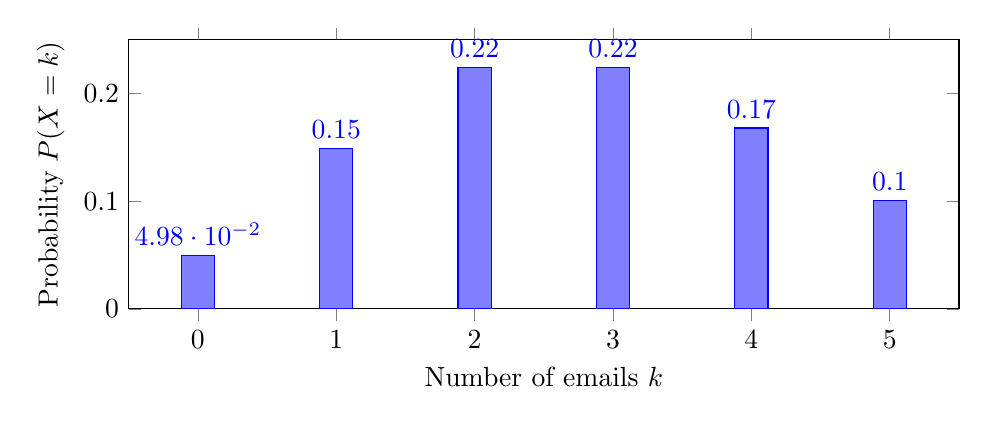
\begin{tikzpicture}
        \begin{axis}[
            ybar,
            bar width=12pt,
            width=\linewidth, height=5cm,
            ymin=0, ymax=0.25,
            xtick=data,
            xlabel={Number of emails \(k\)},
            ylabel={Probability \(P(X=k)\)},
            nodes near coords,
            nodes near coords align={vertical},
          ]
          \addplot+[fill=blue!50] coordinates {
            (0, 0.0498)
            (1, 0.1494)
            (2, 0.2240)
            (3, 0.2240)
            (4, 0.1680)
            (5, 0.1008)
          };
        \end{axis}
      \end{tikzpicture}
    \end{column}
  \end{columns}

\end{frame}


\subsection{Normal distribution}

\begin{frame}{Univariate Gaussian: Definition and Properties}
\textbf{Definition:} A univariate Gaussian (Normal) distribution is defined as:
\[
\mathcal{N}(x \mid \mu, \sigma^2) = \frac{1}{\sqrt{2\pi\sigma^2}} \exp\left( -\frac{(x - \mu)^2}{2\sigma^2} \right)
\]
\textbf{Parameters:}
\begin{itemize}
  \item $\mu$: mean (center of the distribution)
  \item $\sigma^2$: variance (spread of the distribution)
\end{itemize}

\vspace{0.5em}
\textbf{Properties:}
\begin{itemize}
  \item Symmetric around $\mu$
  \item Mean: $\mathbb{E}[x] = \mu$
  \item Variance: $\text{var}[x] = \sigma^2$
\end{itemize}
\end{frame}

\begin{frame}{Univariate Gaussian: Example and Additional Properties}
\textbf{Example:}
\begin{itemize}
  \item Let $x \sim \mathcal{N}(3, 4)$
  \item Then:
    \[
    \mathbb{E}[x] = 3 \qquad \text{var}[x] = 4 \qquad \text{std}[x] = \sqrt{4} = 2
    \]
\end{itemize}

\vspace{0.5em}
\textbf{Additional Properties:}
\begin{itemize}
  \item Linear transformation: If $y = a x + b$, then \\
    $y \sim \mathcal{N}(a\mu + b, a^2\sigma^2)$
  \item Sums of independent Gaussians are Gaussian.
\end{itemize}

\end{frame}



\begin{frame}{Multivariate Gaussian: Definition and Properties}
\textbf{Definition:} A $d$-dimensional multivariate Gaussian is defined as:
\[
\mathcal{N}(\mathbf{x} \mid \boldsymbol{\mu}, \boldsymbol{\Sigma}) =
\frac{1}{(2\pi)^{d/2} |\boldsymbol{\Sigma}|^{1/2}}
\exp\left( -\frac{1}{2} (\mathbf{x} - \boldsymbol{\mu})^\top \boldsymbol{\Sigma}^{-1} (\mathbf{x} - \boldsymbol{\mu}) \right)
\]

\textbf{Parameters:}
\begin{itemize}
  \item $\boldsymbol{\mu} \in \mathbb{R}^d$: mean vector
  \item $\boldsymbol{\Sigma} \in \mathbb{R}^{d \times d}$: covariance matrix
\end{itemize}

\textbf{Mean and Covariance:}
\[
\mathbb{E}[\mathbf{x}] = \boldsymbol{\mu}, \quad \text{Cov}[\mathbf{x}] = \boldsymbol{\Sigma}
\]
\end{frame}

\begin{frame}{Multivariate Gaussian: Example and Key Properties}
\textbf{Example:} Let $\mathbf{x} \sim \mathcal{N} \left(
\begin{bmatrix} 1 \\ 2 \end{bmatrix},
\begin{bmatrix} 2 & 1 \\ 1 & 3 \end{bmatrix}
\right)$

\begin{itemize}
  \item $\boldsymbol{\mu} = \begin{bmatrix} 1 \\ 2 \end{bmatrix}$
  \item $\boldsymbol{\Sigma} = \begin{bmatrix} 2 & 1 \\ 1 & 3 \end{bmatrix}$
\end{itemize}

\vspace{0.5em}
\textbf{Properties:}
\begin{itemize}
  \item Marginals are Gaussian
  \item Affine transformations preserve Gaussianity
  \item If $\mathbf{x}_1$ and $\mathbf{x}_2$ are jointly Gaussian, then $\mathbf{x}_1 \mid \mathbf{x}_2$ is Gaussian
\end{itemize}
\end{frame}

\begin{frame}{Why Are We Obsessed with Gaussians?}

\textbf{Gaussians (a.k.a. Normal distributions) are everywhere:}

\vspace{1em}
\begin{itemize}
  \item \textbf{Mathematically convenient:} Closed-form expressions for mean, variance, marginalization, conditioning, etc.
  \item \textbf{Defined by just two parameters:} Mean $\mu$ and variance (or covariance) $\sigma^2$/$\Sigma$
  \item \textbf{Stable under linear transformations:} Linear combinations of Gaussians are still Gaussian
  \item \textbf{Pop up in nature:} Measurement errors, heights, weights, noise, and many other phenomena
  \item \textbf{Crucial in ML:} Gaussian assumptions simplify models (e.g., Gaussian Naive Bayes, GPs, Kalman filters)
\end{itemize}

\vspace{1em}
\textit{And there is the Central Limit Theorem (CLT)...}

\end{frame}

\subsection{The Central Limit Theorem}

\begin{frame}{The Central Limit Theorem (CLT)}
  \textbf{Why that obsession with Gaussians?}
  \vspace{0.5em}

\textbf{What is the CLT?}
\vspace{0.5em}
If you add up many independent random outcomes,
\textbf{the sum tends to follow a Gaussian distribution.}

\vspace{1em}
\textbf{Why?} Random variation averages out. The “bell curve” emerges naturally when:
\begin{itemize}
  \item Each variable has a \textbf{bounded mean and variance}
  \item The values aren’t too extreme or weird
\end{itemize}

% \vspace{1em}
% \textbf{Important caveats:}
% \begin{itemize}
%   \item ❗ \textbf{Only near the mean:} The approximation breaks down in the tails
%   \item ❗ \textbf{Discrete outcomes:} A sum of integers isn’t truly Gaussian, just close
%   \item ❗ \textbf{Don’t over-trust it:} Use it wisely—don’t assess rare events based on the Gaussian!
% \end{itemize}

\vspace{0.5em}
\textit{We will check that in the exercises later:}
\end{frame}

\begin{frame}{Recap}
  What have we learned so far?

  \begin{itemize}
  \item Distributions and Random Variables are fundamental to model phenomena involving uncertainty.
  \item They are formally defined over a probability space, but we often do not need that formalism in practice; we start directly with a \textbf{distribution}.
  \item The \textbf{expected value} (mean) and \textbf{variance} are key properties of distributions.
  \item Sampling from a distribution is key for estimating the mean and variance.
  \item Some probability distributions are particularly important in probability theory and statistics, e.g., The \textbf{Bernoulli}, \textbf{Poisson}, and \textbf{Gaussian}.
  \end{itemize}
  \vspace{0.5cm}
\end{frame}

\begin{frame}{Recap \& What’s Next}
\textbf{So far, we've seen:}
\begin{itemize}
  \item What probability distributions are.
  \item How they define a \textbf{PDF or PMF}, a \textbf{CDF}, and key properties like \textbf{expectation} and \textbf{variance}.
  \item That we can \textbf{sample} from them to simulate uncertainty.
\end{itemize}

\vspace{1em}
\textbf{What’s missing?} \textit{(Coming next!)}
\begin{itemize}
  \item \textbf{Probabilistic Modeling:}
    \begin{itemize}
      \item How to use distributions to model real-world phenomena.
      \item Introducing \textit{parametric} families (e.g., Normal, Poisson).
    \end{itemize}
  \item \textbf{Probabilistic Inference:}
    \begin{itemize}
      \item How to fit parameters to data.
      \item Via \textit{optimization} or \textit{Bayesian inference}.
      \item Using fitted models to make predictions, decisions, and analyses.
    \end{itemize}
\end{itemize}

\vspace{1em}
\textit{Next time:} From theory to action — modeling, fitting, and applying distributions in machine learning.
\end{frame}


\end{document}
